% Options for packages loaded elsewhere
\PassOptionsToPackage{unicode}{hyperref}
\PassOptionsToPackage{hyphens}{url}
%
\documentclass[
  oneside]{article}
\usepackage{amsmath,amssymb}
\usepackage{iftex}
\ifPDFTeX
  \usepackage[T1]{fontenc}
  \usepackage[utf8]{inputenc}
  \usepackage{textcomp} % provide euro and other symbols
\else % if luatex or xetex
  \usepackage{unicode-math} % this also loads fontspec
  \defaultfontfeatures{Scale=MatchLowercase}
  \defaultfontfeatures[\rmfamily]{Ligatures=TeX,Scale=1}
\fi
\usepackage{lmodern}
\ifPDFTeX\else
  % xetex/luatex font selection
\fi
% Use upquote if available, for straight quotes in verbatim environments
\IfFileExists{upquote.sty}{\usepackage{upquote}}{}
\IfFileExists{microtype.sty}{% use microtype if available
  \usepackage[]{microtype}
  \UseMicrotypeSet[protrusion]{basicmath} % disable protrusion for tt fonts
}{}
\makeatletter
\@ifundefined{KOMAClassName}{% if non-KOMA class
  \IfFileExists{parskip.sty}{%
    \usepackage{parskip}
  }{% else
    \setlength{\parindent}{0pt}
    \setlength{\parskip}{6pt plus 2pt minus 1pt}}
}{% if KOMA class
  \KOMAoptions{parskip=half}}
\makeatother
\usepackage{xcolor}
\usepackage{color}
\usepackage{fancyvrb}
\newcommand{\VerbBar}{|}
\newcommand{\VERB}{\Verb[commandchars=\\\{\}]}
\DefineVerbatimEnvironment{Highlighting}{Verbatim}{commandchars=\\\{\}}
% Add ',fontsize=\small' for more characters per line
\usepackage{framed}
\definecolor{shadecolor}{RGB}{248,248,248}
\newenvironment{Shaded}{\begin{snugshade}}{\end{snugshade}}
\newcommand{\AlertTok}[1]{\textcolor[rgb]{0.94,0.16,0.16}{#1}}
\newcommand{\AnnotationTok}[1]{\textcolor[rgb]{0.56,0.35,0.01}{\textbf{\textit{#1}}}}
\newcommand{\AttributeTok}[1]{\textcolor[rgb]{0.13,0.29,0.53}{#1}}
\newcommand{\BaseNTok}[1]{\textcolor[rgb]{0.00,0.00,0.81}{#1}}
\newcommand{\BuiltInTok}[1]{#1}
\newcommand{\CharTok}[1]{\textcolor[rgb]{0.31,0.60,0.02}{#1}}
\newcommand{\CommentTok}[1]{\textcolor[rgb]{0.56,0.35,0.01}{\textit{#1}}}
\newcommand{\CommentVarTok}[1]{\textcolor[rgb]{0.56,0.35,0.01}{\textbf{\textit{#1}}}}
\newcommand{\ConstantTok}[1]{\textcolor[rgb]{0.56,0.35,0.01}{#1}}
\newcommand{\ControlFlowTok}[1]{\textcolor[rgb]{0.13,0.29,0.53}{\textbf{#1}}}
\newcommand{\DataTypeTok}[1]{\textcolor[rgb]{0.13,0.29,0.53}{#1}}
\newcommand{\DecValTok}[1]{\textcolor[rgb]{0.00,0.00,0.81}{#1}}
\newcommand{\DocumentationTok}[1]{\textcolor[rgb]{0.56,0.35,0.01}{\textbf{\textit{#1}}}}
\newcommand{\ErrorTok}[1]{\textcolor[rgb]{0.64,0.00,0.00}{\textbf{#1}}}
\newcommand{\ExtensionTok}[1]{#1}
\newcommand{\FloatTok}[1]{\textcolor[rgb]{0.00,0.00,0.81}{#1}}
\newcommand{\FunctionTok}[1]{\textcolor[rgb]{0.13,0.29,0.53}{\textbf{#1}}}
\newcommand{\ImportTok}[1]{#1}
\newcommand{\InformationTok}[1]{\textcolor[rgb]{0.56,0.35,0.01}{\textbf{\textit{#1}}}}
\newcommand{\KeywordTok}[1]{\textcolor[rgb]{0.13,0.29,0.53}{\textbf{#1}}}
\newcommand{\NormalTok}[1]{#1}
\newcommand{\OperatorTok}[1]{\textcolor[rgb]{0.81,0.36,0.00}{\textbf{#1}}}
\newcommand{\OtherTok}[1]{\textcolor[rgb]{0.56,0.35,0.01}{#1}}
\newcommand{\PreprocessorTok}[1]{\textcolor[rgb]{0.56,0.35,0.01}{\textit{#1}}}
\newcommand{\RegionMarkerTok}[1]{#1}
\newcommand{\SpecialCharTok}[1]{\textcolor[rgb]{0.81,0.36,0.00}{\textbf{#1}}}
\newcommand{\SpecialStringTok}[1]{\textcolor[rgb]{0.31,0.60,0.02}{#1}}
\newcommand{\StringTok}[1]{\textcolor[rgb]{0.31,0.60,0.02}{#1}}
\newcommand{\VariableTok}[1]{\textcolor[rgb]{0.00,0.00,0.00}{#1}}
\newcommand{\VerbatimStringTok}[1]{\textcolor[rgb]{0.31,0.60,0.02}{#1}}
\newcommand{\WarningTok}[1]{\textcolor[rgb]{0.56,0.35,0.01}{\textbf{\textit{#1}}}}
\usepackage{graphicx}
\makeatletter
\def\maxwidth{\ifdim\Gin@nat@width>\linewidth\linewidth\else\Gin@nat@width\fi}
\def\maxheight{\ifdim\Gin@nat@height>\textheight\textheight\else\Gin@nat@height\fi}
\makeatother
% Scale images if necessary, so that they will not overflow the page
% margins by default, and it is still possible to overwrite the defaults
% using explicit options in \includegraphics[width, height, ...]{}
\setkeys{Gin}{width=\maxwidth,height=\maxheight,keepaspectratio}
% Set default figure placement to htbp
\makeatletter
\def\fps@figure{htbp}
\makeatother
\setlength{\emergencystretch}{3em} % prevent overfull lines
\providecommand{\tightlist}{%
  \setlength{\itemsep}{0pt}\setlength{\parskip}{0pt}}
\setcounter{secnumdepth}{-\maxdimen} % remove section numbering
\newlength{\cslhangindent}
\setlength{\cslhangindent}{1.5em}
\newlength{\csllabelwidth}
\setlength{\csllabelwidth}{3em}
\newlength{\cslentryspacingunit} % times entry-spacing
\setlength{\cslentryspacingunit}{\parskip}
\newenvironment{CSLReferences}[2] % #1 hanging-ident, #2 entry spacing
 {% don't indent paragraphs
  \setlength{\parindent}{0pt}
  % turn on hanging indent if param 1 is 1
  \ifodd #1
  \let\oldpar\par
  \def\par{\hangindent=\cslhangindent\oldpar}
  \fi
  % set entry spacing
  \setlength{\parskip}{#2\cslentryspacingunit}
 }%
 {}
\usepackage{calc}
\newcommand{\CSLBlock}[1]{#1\hfill\break}
\newcommand{\CSLLeftMargin}[1]{\parbox[t]{\csllabelwidth}{#1}}
\newcommand{\CSLRightInline}[1]{\parbox[t]{\linewidth - \csllabelwidth}{#1}\break}
\newcommand{\CSLIndent}[1]{\hspace{\cslhangindent}#1}
\ifLuaTeX
\usepackage[bidi=basic]{babel}
\else
\usepackage[bidi=default]{babel}
\fi
\babelprovide[main,import]{spanish}
% get rid of language-specific shorthands (see #6817):
\let\LanguageShortHands\languageshorthands
\def\languageshorthands#1{}
\usepackage{makeidx}
\makeindex
\usepackage{graphicx}
\usepackage{tikz}
\usepackage{atbegshi}
\usepackage{amsthm}
\newtheorem{definition}{Definición}[section]

\AtBeginDocument{
    \AtBeginShipoutNext{
        \AtBeginShipoutUpperLeft{
            \put(\dimexpr\paperwidth/2-\textwidth/2\relax, -650){
                \makebox[\textwidth]{
                    
\includegraphics[width=0.45\textwidth]{cure_udelar.png}  % Adjust width as needed
                    \hfill
                    
\includegraphics[width=0.405\textwidth]{logoMEDIA.jpeg} % Make it 90% smaller
                }
            }
        }
    }
}
\usepackage{amsthm}
\ifLuaTeX
  \usepackage{selnolig}  % disable illegal ligatures
\fi
\IfFileExists{bookmark.sty}{\usepackage{bookmark}}{\usepackage{hyperref}}
\IfFileExists{xurl.sty}{\usepackage{xurl}}{} % add URL line breaks if available
\urlstyle{same}
\hypersetup{
  pdftitle={Entrega: curso de datos extremales},
  pdfauthor={Laura Montaldo, CI: 3.512.962-7},
  pdflang={es},
  hidelinks,
  pdfcreator={LaTeX via pandoc}}

\title{Entrega: curso de datos extremales}
\author{Laura Montaldo, CI: 3.512.962-7}
\date{2024-03-11}

\begin{document}
\maketitle

\newtheorem{theorem}{Teorema}[section]

\newpage

\thispagestyle{empty}

\maketitle

\newpage

\tableofcontents

\newpage

\hypertarget{resumen}{%
\section{Resumen}\label{resumen}}

Your abstract goes here.

\newpage

\section{Motivación y objetivo del estudio}

Siguiendo a Perera, Segura, y Crisci (2021), se dice que tenemos datos
extremos cuando cada dato corresponde al máximo o mínimo de varios
registros. Son un caso particular de evento raro o gran desviación
respecto a la media. Entonces, en una gran variedad de dominios
disciplinares suele ser de gran interés el trabajo con datos extremos,
los que admiten diversos enfoques. La teoría más clásica de estadística
de datos extremos se basa en los trabajos de Fréchet, Gumbel, Weibull,
Fisher, Tippett, Gnedenko, entre otros. En este estudio, el foco va a
estar puesto en esquemas que extienden a las distribuciones extremales
clásicas.

Los índices de \(S\&P\) son una familia de índices de renta
variable\footnote{En inglés se llaman equity indices} diseñados para
medir el rendimiento del mercado de acciones en Estados Unidos que
cotizan en bolsas estadounidenses. Ésta familia de índices está
compuesta por una amplia variedad de índices basados en tamaño, sector y
estilo. Los índices están ponderados por el criterio
\textit{float-adjusted market capitalization} (FMC). Además, se disponen
de índices ponderados de manera equitativa y con límite de
capitalización de mercado, como es el caso del \(S\&P\:500\). Este este
sentido, el \(S\&P 500\) entraría en el conjunto de índices ponderados
por capitalización bursátil ajustada a la flotación (ver
\href{http://www.overleaf.com}{\textcolor{blue}{$S\&P$ Dow Jones Indices}}).
El mismo mide el rendimiento del segmento de gran capitalización del
mercado estadounidense. Es considerado como un indicador representativo
del mercado de renta variable de los Estados Unidos, y está compuesto
por 500 empresas constituyentes.

Se busca crear un indicador de una posible crisis bursátil. Como
variable de referencia de toma la relación de precios al cierre de ayer
sobre la de hoy

\begin{equation}
Indicador_t=\frac{Precio_{t-1}}{Precio_t},\quad\text{para}\; t=1,...,T \label{eq:ind}
\end{equation} \vspace{0.5cm}

Interpretación del Indicador:

\begin{itemize}
\item Si el $Indicador_t$    $\leq$ 1, el precio de cierre de hoy es mayor o igual que el de ayer, lo cual podría ser considerado una señal positiva.
\item Si el $Indicador_t$ > 1, el precio de cierre de hoy es menor que el de ayer, lo cual podría considerarse una señal de alerta.
\end{itemize}

\vspace{1cm}

\newpage

En las siguiente figuras se muestra la evolución histórica desde la
fecha 03/01/1928 hasta 08/12/2023 del precio al cierre del día del
indicar S\&P 500.

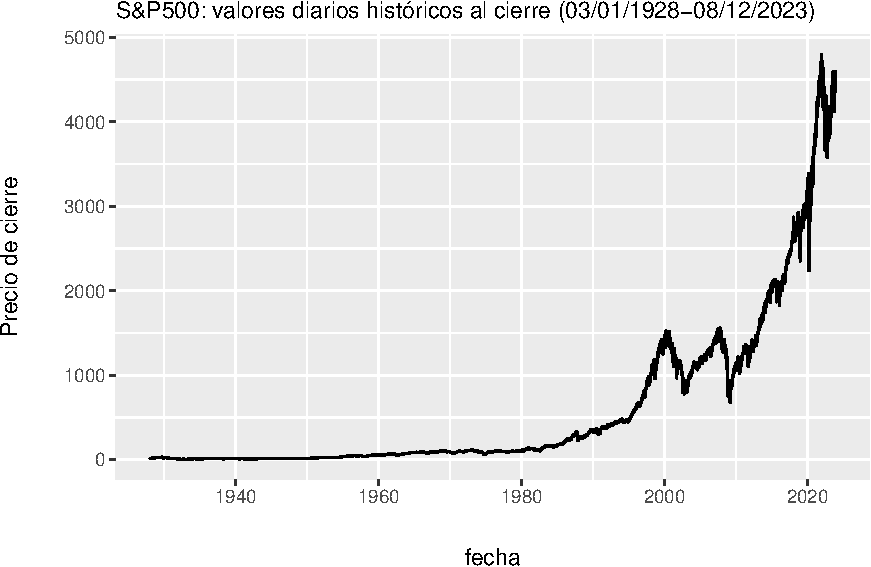
\includegraphics{main_files/figure-latex/plot1-1.pdf}

\begin{verbatim}
## [1] 24100     9
\end{verbatim}

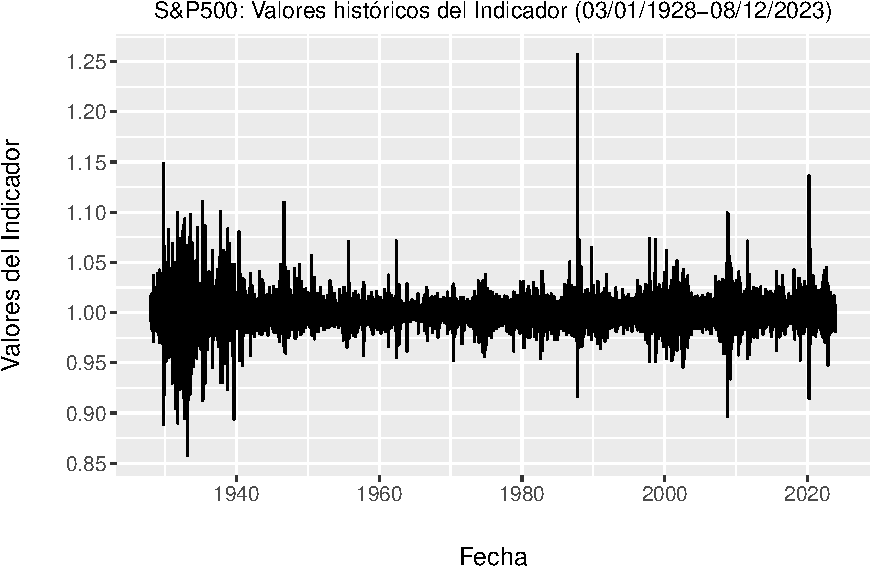
\includegraphics{main_files/figure-latex/unnamed-chunk-13-1.pdf}

\begin{Shaded}
\begin{Highlighting}[]
\NormalTok{ts\_relacion}\OtherTok{=}\NormalTok{df[,}\FunctionTok{c}\NormalTok{(}\StringTok{\textquotesingle{}relacion\textquotesingle{}}\NormalTok{)]}
\end{Highlighting}
\end{Shaded}

\begin{Shaded}
\begin{Highlighting}[]
\NormalTok{result\_adf }\OtherTok{\textless{}{-}} \FunctionTok{suppressWarnings}\NormalTok{(}\FunctionTok{adf.test}\NormalTok{(ts\_relacion))}
\FunctionTok{cat}\NormalTok{(}\StringTok{\textquotesingle{}p{-}valor adf:\textquotesingle{}}\NormalTok{, result\_adf}\SpecialCharTok{$}\NormalTok{p.value ,}\StringTok{\textquotesingle{}}\SpecialCharTok{\textbackslash{}n}\StringTok{\textquotesingle{}}\NormalTok{)}
\end{Highlighting}
\end{Shaded}

\begin{verbatim}
## p-valor adf: 0.01
\end{verbatim}

\begin{Shaded}
\begin{Highlighting}[]
\NormalTok{result\_kpss }\OtherTok{\textless{}{-}} \FunctionTok{suppressWarnings}\NormalTok{(}\FunctionTok{kpss.test}\NormalTok{(ts\_relacion))}
\FunctionTok{cat}\NormalTok{(}\StringTok{\textquotesingle{}p{-}valor kpss:\textquotesingle{}}\NormalTok{, result\_kpss}\SpecialCharTok{$}\NormalTok{p.value ,}\StringTok{\textquotesingle{}}\SpecialCharTok{\textbackslash{}n}\StringTok{\textquotesingle{}}\NormalTok{)}
\end{Highlighting}
\end{Shaded}

\begin{verbatim}
## p-valor kpss: 0.1
\end{verbatim}

\begin{Shaded}
\begin{Highlighting}[]
\CommentTok{\#install.packages(\textquotesingle{}aTSA\textquotesingle{})}
\NormalTok{aTSA}\SpecialCharTok{::}\FunctionTok{adf.test}\NormalTok{(ts\_relacion)}
\end{Highlighting}
\end{Shaded}

\begin{verbatim}
## Augmented Dickey-Fuller Test 
## alternative: stationary 
##  
## Type 1: no drift no trend 
##       lag    ADF p.value
##  [1,]   0 -1.326   0.205
##  [2,]   1 -0.770   0.404
##  [3,]   2 -0.543   0.486
##  [4,]   3 -0.414   0.525
##  [5,]   4 -0.340   0.547
##  [6,]   5 -0.298   0.559
##  [7,]   6 -0.255   0.571
##  [8,]   7 -0.221   0.581
##  [9,]   8 -0.190   0.590
## [10,]   9 -0.180   0.593
## [11,]  10 -0.164   0.597
## [12,]  11 -0.152   0.601
## [13,]  12 -0.141   0.604
## [14,]  13 -0.128   0.608
## Type 2: with drift no trend 
##       lag    ADF p.value
##  [1,]   0 -156.9    0.01
##  [2,]   1 -112.1    0.01
##  [3,]   2  -90.6    0.01
##  [4,]   3  -77.8    0.01
##  [5,]   4  -68.9    0.01
##  [6,]   5  -64.6    0.01
##  [7,]   6  -58.9    0.01
##  [8,]   7  -54.7    0.01
##  [9,]   8  -50.2    0.01
## [10,]   9  -47.2    0.01
## [11,]  10  -44.8    0.01
## [12,]  11  -42.6    0.01
## [13,]  12  -41.9    0.01
## [14,]  13  -40.1    0.01
## Type 3: with drift and trend 
##       lag    ADF p.value
##  [1,]   0 -156.9    0.01
##  [2,]   1 -112.1    0.01
##  [3,]   2  -90.6    0.01
##  [4,]   3  -77.8    0.01
##  [5,]   4  -68.9    0.01
##  [6,]   5  -64.7    0.01
##  [7,]   6  -59.0    0.01
##  [8,]   7  -54.7    0.01
##  [9,]   8  -50.2    0.01
## [10,]   9  -47.2    0.01
## [11,]  10  -44.9    0.01
## [12,]  11  -42.6    0.01
## [13,]  12  -41.9    0.01
## [14,]  13  -40.1    0.01
## ---- 
## Note: in fact, p.value = 0.01 means p.value <= 0.01
\end{verbatim}

\newpage

\section{Marco teorico}
\subsection{El enfoque de conteo de eventos y los modelos de base Poissoniana.}

Fijaremos un cierto umbral, llamaremos \textit{evento} cuando la
variable observada supera ese umbral y dado un cierto intervalo del
tiempo \(J\), contaremos

\textbackslash begin\{eqution\} N(J)=
\text{número de eventos en el intervalo}; J.
\textbackslash end\{equation\}

Fijando un \(u=1.025\), el evento es una señal negativa del precio de
\(SP\$500\) que estaría dado por la cantidad de días en el mes \(J\) que
\(Indicador_t\) supera el umbral \(u\). Un evento ser que
\(Indicador_t\) supere un umbral \(u>1.025\). Si el número de eventos
está dado por los días de un mes, entonces \(N(mes)\) va a ser la
cantidad de días que occurió el evento en un mes, \(N(mes)=3\) es la
cantidad de señales negativas en el mes.

como la cantidad de días (\(d\)) que el indicar aumentó un cierto
porcentaje de \(d-1\) a \(d\).

\(2.5\%\) en un Si \(d\) es la cantidad de días y \(J\) es el intervalo
de días en un mes, N(mes) N(mes)= cantidad de períodos de 3 días durante
un mes, en que se registró una aumento mayor o igual a 2.5\% del índice
de un día para el otro.

\(N\) es lo que se llama un proceso de conteo o proceso
puntua\footnote{\textit{Counting process, Point process} en inglés}, un
tipo de modelos utilizados en Logística, Telecomunicaciones, estudios de
Contaminación Atmosférica o Costera, Clima, etc.

El proceso de conteo más simple es el llamado
\textit{Proceso de Poisson}, que puede caracterizarse de la siguiente
manera.

\begin{definition}[Proceso de Poisson]\label{def:1}
Si $N$ es un proceso de conteo y $\lambda>0$, diremos que $N$ es un Proceso de Poisson de parámetro $\lambda$ (y abreviaremos $N$ es $PP(\lambda)$ ) si se cumple:
\begin{itemize}
\item[a)] Para todo intervalo $J$ de los reales positivos, $N(J)$ es una variable aleatoria que tiene distribución de Poisson de parámetro $\lambda$ longitud($J$).
\item[b)] Si $J, L, M...$ es una cantidad arbitraria de intervalos de reales positivos \textit{disjuntos}, entonces $N(J), N(L), N(M),...$ son variables aleatorias independientes.
\end{itemize}
\end{definition}

El siguiente teorema brinda una visualización muy interesante de los
Procesos de Poisson, que nos servirá mucho para introducir otros modelos
y que es ideal para poder simular computacionalmente Procesos de
Poissson.

\begin{theorem}[Otra visión de los Procesos de Poisson]\label{thm:otra_vision}
Si $T_1,...,T_n,...$ se supone $iid$,  con distribución Exponencial de parámetro $\lambda>0$ y definimos que ocurre el primer evento en el instante $T_1$, el segundo en el instante $T_1+T_2$, el tercero en el instante $T_1+T_2+T_3$ y asì sucesivamente, el proceso $N$ de conteo de tales eventos, es un proceso de Poisson.
\end{theorem}

Dicho de otro modo el Proceso de Poisson representa eventos aislados
(``que ocurren de a uno y claramente separados''), con tiempos
inter-eventos \(iid\) y exponenciales. Obviamente, esto muchas veces es
\textit{too good to be true}, pero variaciones de este modelo tan simple
pueden brindar modelos realistas.

\hypertarget{observaciuxf3n-1}{%
\subparagraph{Observación 1:}\label{observaciuxf3n-1}}

En la práctica, si se toman datos en los instantes \(1,...,n\) suele
reescalarse el tiempo dividiendo por \(n\) y los instantes quedan en
\([0,1]\). Allí se define un \(PP\) de manera casi idéntica, obviamente
modificando en la definición, tanto en \(a)\) como en \(b)\) que los
intervalos deben estar contenidos en \([0,1]\).

\hypertarget{observaciuxf3n-2}{%
\subparagraph{Observación 2:}\label{observaciuxf3n-2}}

Conviene recordar que si \(X\) es una \(VA\) Poisson de parámetro
\(\lambda>0\) y \(T\) es una \(VA\) exponencial de parámetro
\(\lambda\), entonces \(E(X)= \lambda\) y \(E(T)=1/lambda\) . Si
\(T_1,...,T_n,...\) siendo \(iid\) son los tiempos inter-eventos de un
\(PP(\lambda)\) se deduce entonces de la ley de los grandes números que

\begin{equation}
\frac{\sum_{i=1}^{i=n} T_i}{n} \rightarrow 1/ \lambda \quad cuando \quad n\rightarrow \infty
\end{equation}

Es decir que el tiempo promedio entre eventos ``a la larga'' es
\(1/\lambda\) . Similarmente si \(J_1,...,J_n,...\) son intervalos
disjuntos de longitud \(1\), por la definición \ref{def:1} y la ley de
los grandes números se tiene que

\begin{equation}
\frac{\sum_{i=1}^{i=n} N(J_i)}{n} \rightarrow \lambda \quad cuando \quad n\rightarrow \infty
\end{equation}

Más aún, puede probarse que

\begin{equation}
\frac{N((0,t))}{t} \rightarrow \lambda \quad cuando \quad t \rightarrow \infty
\end{equation}

Esto permite observar una consecuencia del Teorema
\ref{thm:otra_vision}, que es una propiedad intuitivamente muy
atractiva.

La tasa promedial de incidencia de los eventos en un \(PP(\lambda)\) es
inversamente proporcional al tiempo promedial inter-eventos.

\hypertarget{ejemplo-1}{%
\subparagraph{Ejemplo 1:}\label{ejemplo-1}}

Propiedades como esta hicieron, en las primeras dos décadas del siglo
\(XX\), a un creador genial como Agner Erlang modelar mediante Procesos
de Poisson las llamadas que arribaban a una central telefónica, así como
(con parámetros muy distintos) el proceso de ocupación de las líneas
entre dos centrales. Eso condujo no sólo al desarrollo de las primeras
centrales de telefonía conmutada por circuitos por CTC, la filial danesa
de Bell, sino además a que Erlang desarrollara su ``fórmulas de
bloqueo'', fino cálculo por el cual, según los parámetros del proceso de
arribo y del proceso de ocupación de líneas, se calcula la probabilidad
de ``saturación'' (no hay ninguna línea disponible) dado el número de
líneas entre centrales, o, dada una probabilidad de saturación
``tolerable'' (\(\epsilon\)).

DISEÑAR (determinar el mínimo número de lineas necesarias para que la
probabilidad de bloqueo no exceda \(\epsilon\) ). Si el tiempo entre
arribos de llamadas a la central es Exponencial de parámetro
\(\lambda\), y la duración media de una llamada es Exponencial de
parámetro \(\mu\), entonces el parámetro crucial de la fórmula de Erlang
es

\begin{align}
\rho=&\lambda/\mu  \nonumber \\
= &\text{“duración media de la llamada”/ “tiempo medio entre llamadas”}\label{eq:ro}
\end{align}

y a mayor valor de \(\rho\), mayor probabilidad de saturación para una
conectividad dada. Esta fórmula \eqref{eq:ro} aún sigue en uso en
algunos problemas y dió pie al desarrollo de fórmulas de bloqueo más
sofisticadas para situaciones más complejas. Con mucha justicia, la
unidad en la que se mide la intensidad de tráfico en redes se llama
\textit{erlang} y este ejemplo nos parece una clara muestra de cuán útil
ha sido el muy sencillo Proceso de Poisson. Sin embargo, en otros
problemas, por ejemplo en modernas redes de datos en las que los
``eventos'' de ``demanda de servicio'' pueden ocurrir simultáneamente en
muy grandes cantidades (``clustering''), aparece un modelo más
sofisticado, que puede ser definido a partir del Proceso de Poisson: el
Proceso de Poisson Compuesto.

\begin{definition}[Proceso de Poisson Compuesto]\label{def:2}
Si $N$ es un Proceso de Poisson de parámetro $\lambda>0$ , $G$ es una distribución de probabilidad en los naturales $1,2,3...$, consideramos un proceso $S_1,...,S_n$ $iid$ con distribución $G$ y construímos un nuevo proceso de conteo $M$ de la forma siguiente:
\begin{itemize}
\item Cuando $N$ tiene su primer evento, $M$ tiene $S_1$ eventos simultáneos;
\item Cuando $N$ tiene su segundo evento, $M$ tiene $S_2$ eventos simultáneos..... (y así sucesivamente)
\end{itemize}
decimos que $M$ es un Proceso de Poisson Compuesto de parámetro $\lambda>0$ y distribución de eventos $G$ (y abreviaremos $M$ es $PPC(\lambda;G)$)
\end{definition}

\hypertarget{ejercicio-1}{%
\subparagraph{Ejercicio 1 :}\label{ejercicio-1}}

Demostrar que para un \(PPC(\lambda;G)\) el tiempo medio inter-eventos
sigue siendo \(1/\lambda\), pero que la tasa de incidencia media de
eventos ahora es \(lambda E(G)\).

\hypertarget{observaciuxf3n-3.}{%
\subparagraph{Observación 3.}\label{observaciuxf3n-3.}}

Para aclarar, si \(G\) es una distribución degenerada otorga al 1
probabilidad 1, el correspondiente \(PPC(\lambda;G)\) en realidad es un
\(PPC(\lambda)\). Ergo, el \(PP\) es un caso particular de \(PPC\).

\hypertarget{observaciuxf3n-4.}{%
\subparagraph{Observación 4.}\label{observaciuxf3n-4.}}

Para evitar confusiones frecuentes, distinguiremos explícitamente estos
procesos de los llamados Procesos de Poisson no-homogéneos. Para ello
recordemos, sin entrar en tecnicismos, que una medida en los reales
positivos es una función que a los conjuntos asocia números positivos
con las mismas propiedades formales, excepto que no tiene por qué dar a
todo el conjunto de los reales positivos ( a todo el universo) el valor
1. Dicho de otro modo una probabilidad es una medida particular, que a
todo el universo asigna el valor 1. Puede pensarse como ejemplo típico
de una medida, la que asigna a un conjunto la integral sobre ese
conjunto de una función no negativa (no necesariamente de integral total
1, puede ser incluso infinita). La longitud es el ejemplo más simple de
medida (llamada también medida de Lebesgue) y la longitud de todos los
reales positivos es infinito. Puede demostrarse que la longitud
multiplicada por una constante no negativa son las únicas medidas
invariantes por traslaciones, punto importante para la distinción que
queremos hacer.

\begin{definition}[Proceso de Poisson No Homogéneo]\label{def:3}
Si $N$ es un proceso de conteo y $m$ es una medida que NO puede expresarse como una constante por la longitud, diremos que $N$ es un Proceso de Poisson No Homogéneo de medida $m$ (y abreviaremos $N$ es $PPNH(m)$ ) si se cumple:

\begin{itemize}
\item[a)] Para todo intervalo $J$ de los reales positivos, $N(J)$ es una variable aleatoria que tiene distribución de Poisson de parámetro $m(J)$.
\item[b)] Si $J, L, M...$ es una cantidad arbitraria de intervalos positivos DISJUNTOS, entonces $N(J), N(L), N(M),...$ son variables aleatorias independientes.
\end{itemize}
\end{definition}

Queda claro que el proceso de Poisson podría verse de la manera a) y b)
anterior cuando \(m=\text{constante por longitud}\), por eso, para no
confundir, se excluye a título expreso que \(m\) pueda ser constante por
longitud. Para dejar en claro la diferencia entre los PPNH y los PPC ( o
el simple PP), recordemos que en los PPC, los tiempos inter-eventos son
exponenciales de parámetro \(\lambda>0\) e \(iid\). El siguiente
resultado muestra la diferencia de conceptos. Por su extrema
simplicidad, lo detallaremos.

\begin{theorem}[PPNH no es PPC]\label{thm:2}
Si $N$ es un PPNH y $T_1$ es el tiempo del primer evento, la distribución de $T_1$ no es exponencial.
Por lo tanto, un PPNH no es PPC.
\end{theorem}

\hypertarget{demostraciuxf3n}{%
\subparagraph{Demostración:}\label{demostraciuxf3n}}

\[
P(T_1\le t)=P(N((0,t))\ge 1)=1-P(N((0,t))=0)= 1-e^{-m((0,t))}\quad\text{para todo}\; t>0.
\]

Si \(T_1\) fuera exponencial, entonces para algún \(\lambda>0\) y para
todo \(t>0\) sería:

\(m((0,t))= \lambda t\) y por ende, si \(a <b\) cualquiera,

\[m((a,b))= m((0,b))-m((0,a))=\lambda b- \lambda a= \lambda(b-a)=\lambda x\;longitud((a,b))\]

por lo cual se concluye, \(m=\lambda x\:longitud\)

lo cual es absurdo \(\blacklozenge\).

\newpage

\subsection{POT (Peaks Over Treshold) y variantes}

\newpage
\section{Estrategia Empírica}

A la columna relativa a la relacion de precios se la resta por 1 para
tener centrados los valores de la relacion de precios en cero. Y
posteriormente analizar si las series, fijando distintos umbrales son
estacionarias.

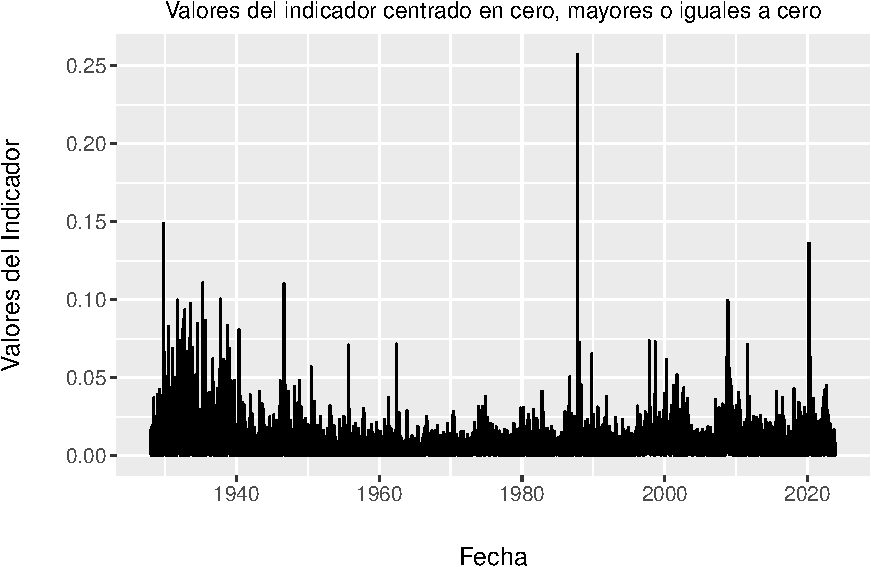
\includegraphics{main_files/figure-latex/unnamed-chunk-21-1.pdf}

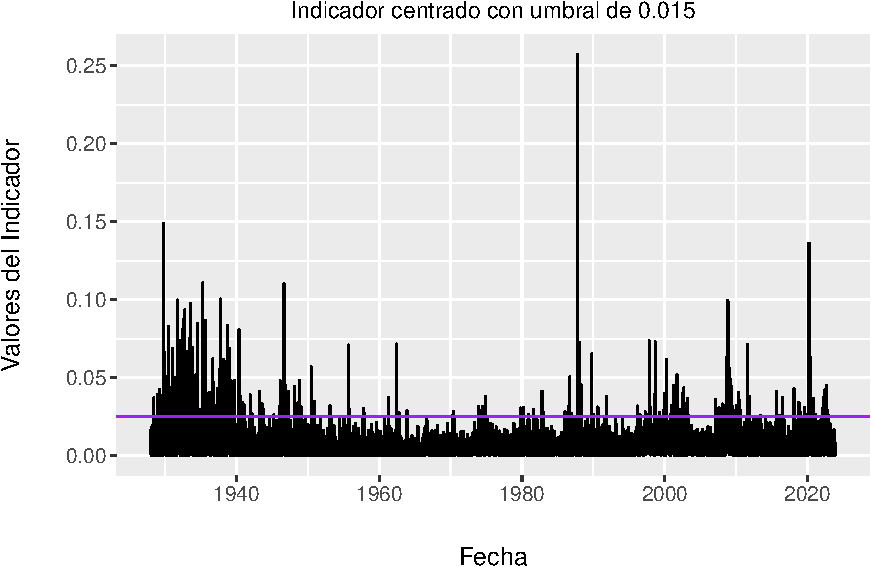
\includegraphics{main_files/figure-latex/unnamed-chunk-22-1.pdf}

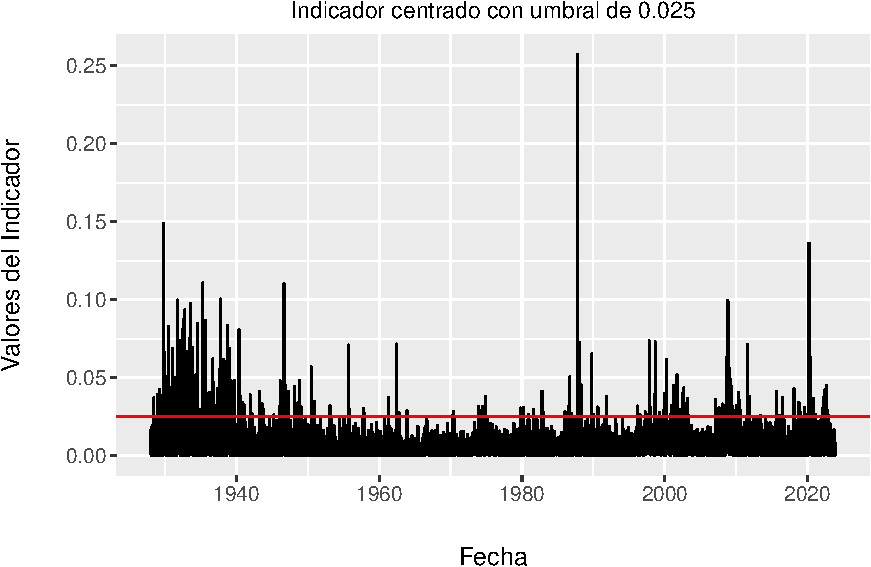
\includegraphics{main_files/figure-latex/unnamed-chunk-23-1.pdf}

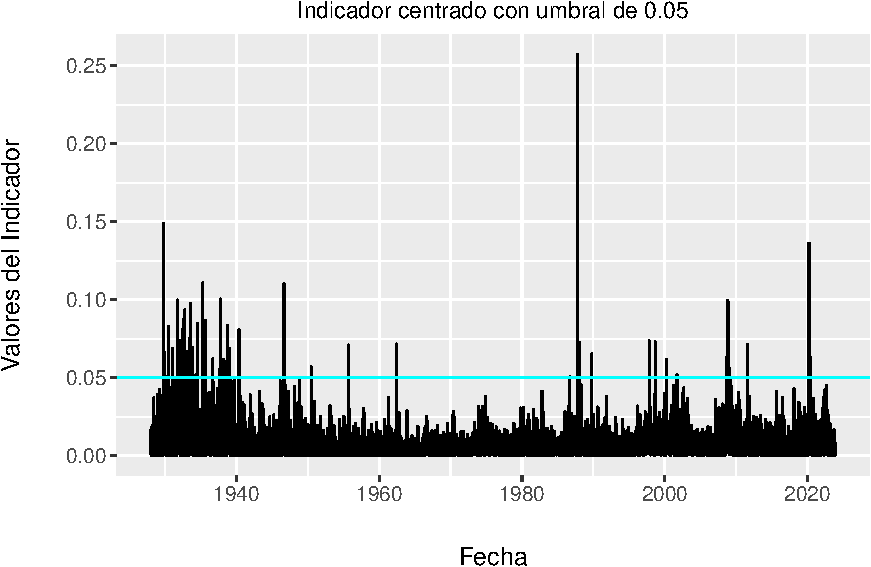
\includegraphics{main_files/figure-latex/unnamed-chunk-24-1.pdf}

\begin{Shaded}
\begin{Highlighting}[]
\NormalTok{filtered\_df\_0\_025 }\OtherTok{\textless{}{-}}\NormalTok{ df }\SpecialCharTok{\%\textgreater{}\%}
  \FunctionTok{filter}\NormalTok{(rel\_cero}\SpecialCharTok{\textgreater{}=} \FloatTok{0.025}\NormalTok{)}
\end{Highlighting}
\end{Shaded}

\begin{Shaded}
\begin{Highlighting}[]
\FunctionTok{head}\NormalTok{(filtered\_df\_0\_025)}
\end{Highlighting}
\end{Shaded}

\begin{verbatim}
##         Date  Open  High   Low Close Volume Dividends Stock.Splits relacion
## 1 1928-06-11 18.68 18.68 18.68 18.68      0         0            0 1.036938
## 2 1928-07-11 18.95 18.95 18.95 18.95      0         0            0 1.025330
## 3 1928-12-06 22.91 22.91 22.91 22.91      0         0            0 1.039284
## 4 1929-02-07 24.71 24.71 24.71 24.71      0         0            0 1.031566
## 5 1929-03-25 24.51 24.51 24.51 24.51      0         0            0 1.042432
## 6 1929-04-01 24.88 24.88 24.88 24.88      0         0            0 1.026125
##     rel_cero
## 1 0.03693793
## 2 0.02532979
## 3 0.03928414
## 4 0.03156620
## 5 0.04243162
## 6 0.02612546
\end{verbatim}

\begin{Shaded}
\begin{Highlighting}[]
\NormalTok{data}\OtherTok{=}\NormalTok{filtered\_df\_0\_025[,}\FunctionTok{c}\NormalTok{(}\StringTok{\textquotesingle{}Date\textquotesingle{}}\NormalTok{, }\StringTok{\textquotesingle{}rel\_cero\textquotesingle{}}\NormalTok{)]}
\NormalTok{n}\OtherTok{=}\FunctionTok{dim}\NormalTok{(data)[}\DecValTok{1}\NormalTok{]}
\end{Highlighting}
\end{Shaded}

\begin{Shaded}
\begin{Highlighting}[]
\NormalTok{fecha\_maxima }\OtherTok{\textless{}{-}} \FunctionTok{max}\NormalTok{(data}\SpecialCharTok{$}\NormalTok{Date)}
\CommentTok{\# Reescalar el tiempo dividiendo cada fecha por la fecha máxima}
\NormalTok{data}\SpecialCharTok{$}\NormalTok{tiempo\_reescalado }\OtherTok{\textless{}{-}} \FunctionTok{as.numeric}\NormalTok{(data}\SpecialCharTok{$}\NormalTok{Date }\SpecialCharTok{{-}} \FunctionTok{min}\NormalTok{(data}\SpecialCharTok{$}\NormalTok{Date)) }\SpecialCharTok{/} \FunctionTok{as.numeric}\NormalTok{(fecha\_maxima }\SpecialCharTok{{-}} \FunctionTok{min}\NormalTok{(data}\SpecialCharTok{$}\NormalTok{Date))}
\FunctionTok{head}\NormalTok{(data)}
\end{Highlighting}
\end{Shaded}

\begin{verbatim}
##         Date   rel_cero tiempo_reescalado
## 1 1928-06-11 0.03693793      0.0000000000
## 2 1928-07-11 0.02532979      0.0008690614
## 3 1928-12-06 0.03928414      0.0051564311
## 4 1929-02-07 0.03156620      0.0069814600
## 5 1929-03-25 0.04243162      0.0083140209
## 6 1929-04-01 0.02612546      0.0085168019
\end{verbatim}

\begin{Shaded}
\begin{Highlighting}[]
\FunctionTok{ggplot}\NormalTok{(df, }\FunctionTok{aes}\NormalTok{(}\AttributeTok{x =}\NormalTok{ Date, }\AttributeTok{y =}\NormalTok{ rel\_cero)) }\SpecialCharTok{+}
  \FunctionTok{geom\_line}\NormalTok{() }\SpecialCharTok{+}
  \FunctionTok{geom\_hline}\NormalTok{(}\AttributeTok{yintercept =} \FloatTok{0.05}\NormalTok{, }\AttributeTok{linetype =} \StringTok{"solid"}\NormalTok{, }\AttributeTok{color =} \StringTok{"cyan"}\NormalTok{) }\SpecialCharTok{+}  \CommentTok{\# Add horizontal line}
  \FunctionTok{ggtitle}\NormalTok{(}\StringTok{"S\&P500: Valores históricos del Indicador (03/01/1928{-}08/12/2023)"}\NormalTok{) }\SpecialCharTok{+}
  \FunctionTok{xlab}\NormalTok{(}\StringTok{"Fecha"}\NormalTok{) }\SpecialCharTok{+}
  \FunctionTok{ylab}\NormalTok{(}\StringTok{"Valores del Indicador"}\NormalTok{) }\SpecialCharTok{+}
  \FunctionTok{scale\_x\_date}\NormalTok{(}\AttributeTok{limits =}\NormalTok{ date\_range) }\SpecialCharTok{+}
  \FunctionTok{scale\_y\_continuous}\NormalTok{(}\AttributeTok{breaks =} \FunctionTok{seq}\NormalTok{(}\DecValTok{0}\NormalTok{, }\FunctionTok{ceiling}\NormalTok{(}\FunctionTok{max}\NormalTok{(df}\SpecialCharTok{$}\NormalTok{relacion)), }\AttributeTok{by =} \FloatTok{0.05}\NormalTok{)) }\SpecialCharTok{+}
  \FunctionTok{theme}\NormalTok{(}
    \AttributeTok{axis.title.x =} \FunctionTok{element\_text}\NormalTok{(}\AttributeTok{margin =} \FunctionTok{margin}\NormalTok{(}\AttributeTok{t =} \DecValTok{20}\NormalTok{, }\AttributeTok{b =} \DecValTok{40}\NormalTok{)),}
    \AttributeTok{axis.title.y =} \FunctionTok{element\_text}\NormalTok{(}\AttributeTok{margin =} \FunctionTok{margin}\NormalTok{(}\AttributeTok{r =} \DecValTok{20}\NormalTok{, }\AttributeTok{l =} \DecValTok{40}\NormalTok{)),}
    \AttributeTok{plot.title =} \FunctionTok{element\_text}\NormalTok{(}\AttributeTok{size =} \DecValTok{11}\NormalTok{, }\AttributeTok{hjust =} \FloatTok{0.5}\NormalTok{),  }\CommentTok{\# Center the plot title}
    \AttributeTok{axis.text =} \FunctionTok{element\_text}\NormalTok{(}\AttributeTok{size =} \DecValTok{10}\NormalTok{),  }\CommentTok{\# Adjust the size of axis text}
    \AttributeTok{axis.title =} \FunctionTok{element\_text}\NormalTok{(}\AttributeTok{size =} \DecValTok{12}\NormalTok{),  }\CommentTok{\# Adjust the size of axis titles}
    \AttributeTok{legend.title =} \FunctionTok{element\_text}\NormalTok{(}\AttributeTok{size =} \DecValTok{10}\NormalTok{),  }\CommentTok{\# Adjust the size of legend title}
    \AttributeTok{legend.text =} \FunctionTok{element\_text}\NormalTok{(}\AttributeTok{size =} \DecValTok{8}\NormalTok{)  }\CommentTok{\# Adjust the size of legend text}
\NormalTok{  )}
\end{Highlighting}
\end{Shaded}

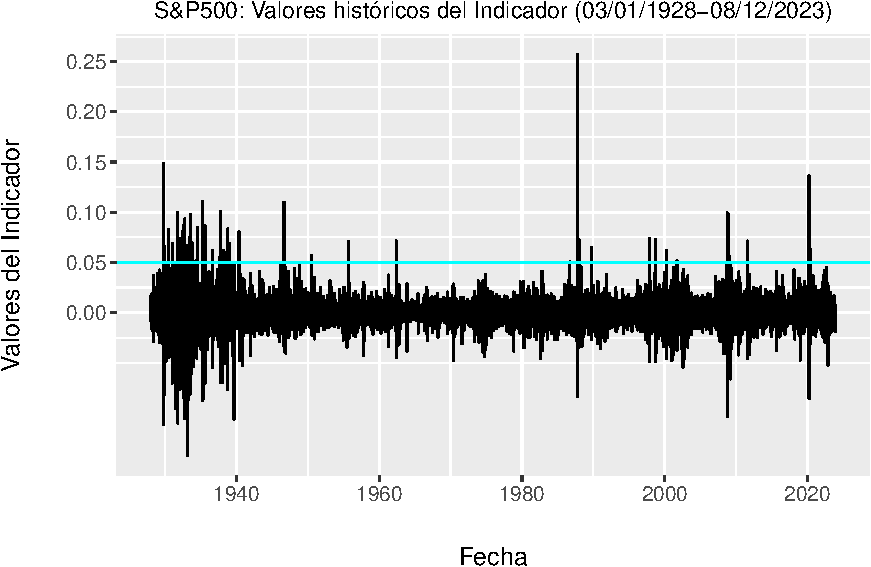
\includegraphics{main_files/figure-latex/unnamed-chunk-28-1.pdf}

\begin{Shaded}
\begin{Highlighting}[]
\NormalTok{filtered\_df\_0\_05 }\OtherTok{\textless{}{-}}\NormalTok{ df }\SpecialCharTok{\%\textgreater{}\%}
  \FunctionTok{filter}\NormalTok{(rel\_cero }\SpecialCharTok{\textgreater{}=} \FloatTok{0.05}\NormalTok{)}
\FunctionTok{dim}\NormalTok{(filtered\_df\_0\_05)}
\end{Highlighting}
\end{Shaded}

\begin{verbatim}
## [1] 98 10
\end{verbatim}

\begin{Shaded}
\begin{Highlighting}[]
\FunctionTok{plot}\NormalTok{(filtered\_df\_0\_05)}
\end{Highlighting}
\end{Shaded}

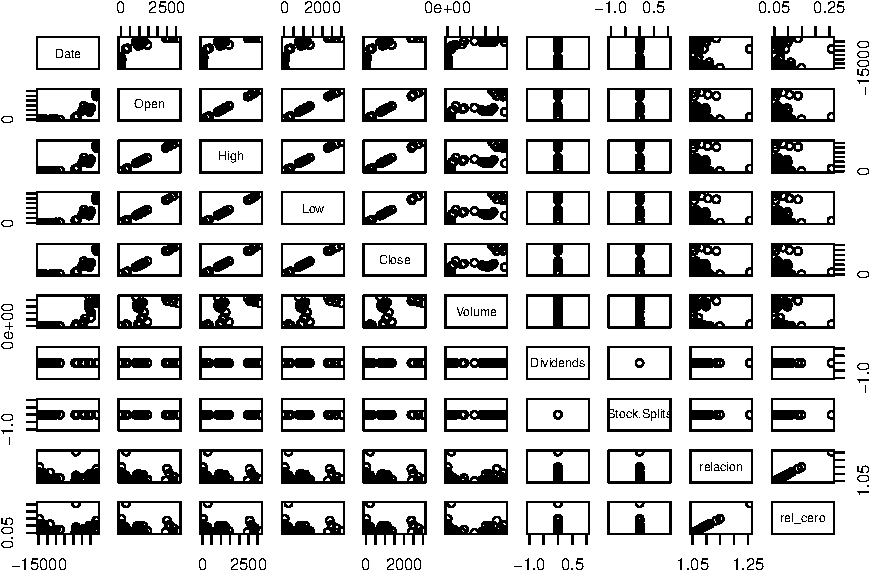
\includegraphics{main_files/figure-latex/unnamed-chunk-30-1.pdf}

\begin{Shaded}
\begin{Highlighting}[]
\FunctionTok{hist}\NormalTok{(filtered\_df\_0\_05}\SpecialCharTok{$}\NormalTok{relacion, }\AttributeTok{main =} \StringTok{"Histograma relacion con umbral 0.05 "}\NormalTok{, }\AttributeTok{xlab =} \StringTok{"relacion"}\NormalTok{)}
\end{Highlighting}
\end{Shaded}

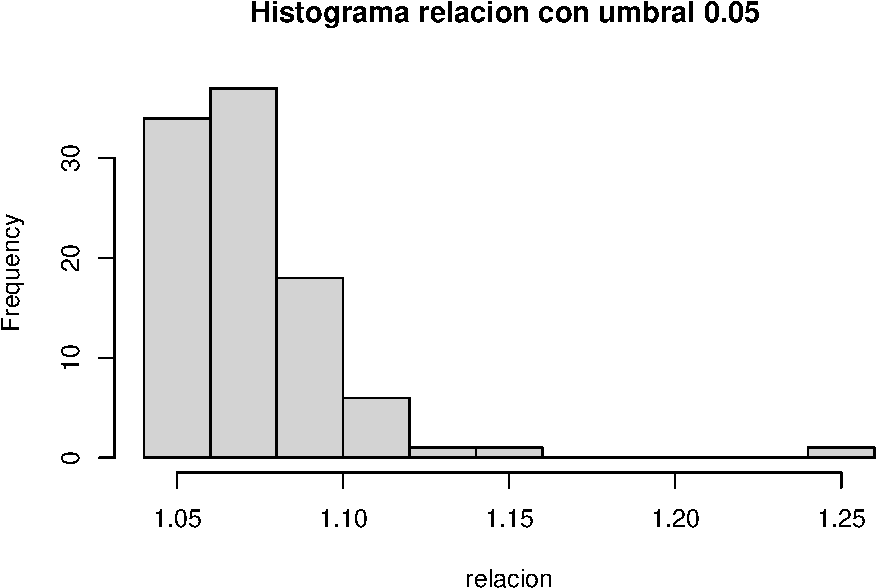
\includegraphics{main_files/figure-latex/unnamed-chunk-31-1.pdf}

\begin{Shaded}
\begin{Highlighting}[]
\FunctionTok{hist}\NormalTok{(filtered\_df\_0\_025}\SpecialCharTok{$}\NormalTok{relacion, }\AttributeTok{main =} \StringTok{"Histograma relacion con umbral 0.025 "}\NormalTok{, }\AttributeTok{xlab =} \StringTok{"relacion"}\NormalTok{)}
\end{Highlighting}
\end{Shaded}

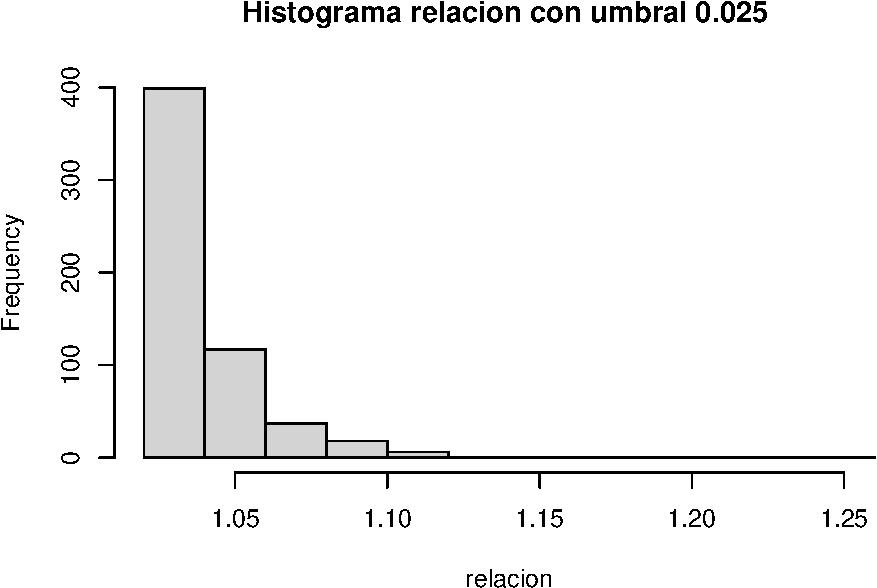
\includegraphics{main_files/figure-latex/unnamed-chunk-32-1.pdf}

\hypertarget{refs}{}
\begin{CSLReferences}{1}{0}
\leavevmode\vadjust pre{\hypertarget{ref-enders}{}}%
Enders, W. 2014. \emph{Applied Econometric Time Series}. Wiley Series en
Probability y Statistics. Wiley.

\leavevmode\vadjust pre{\hypertarget{ref-notas_curso}{}}%
Perera, Gonzalo, Angel Segura, y Carolina Crisci. 2021. \emph{Curso de
estadística de datos extremales, cap. 1 a cap. 5}.

\leavevmode\vadjust pre{\hypertarget{ref-kpss}{}}%
Shin, Yongcheol, Denis Kwiatkowski, Peter Schmidt, y Peter C. B.
Phillips. 1992. {«Testing the Null Hypothesis of Stationarity Against
the Alternative of a Unit Root: How Sure Are We That Economic Time
Series Are Nonstationary?»} \emph{Journal of Econometrics} 54 (1-3):
159-78.

\leavevmode\vadjust pre{\hypertarget{ref-evd}{}}%
Stephenson, A. G. 2002. {«evd: Extreme Value Distributions»}. \emph{R
News} 2 (2): 0. \url{https://CRAN.R-project.org/doc/Rnews/}.

\end{CSLReferences}

\end{document}
